%%%%%%%%%%%%%%%%%%%%%%%%%%%%%%%%%%%%%%%%%
% Beamer Presentation
% LaTeX Template
% Version 1.0 (10/11/12)
%
% This template has been downloaded from:
% http://www.LaTeXTemplates.com
%
% License:
% CC BY-NC-SA 3.0 (http://creativecommons.org/licenses/by-nc-sa/3.0/)
%
%%%%%%%%%%%%%%%%%%%%%%%%%%%%%%%%%%%%%%%%%

%----------------------------------------------------------------------------------------
%	PACKAGES AND THEMES
%----------------------------------------------------------------------------------------

\documentclass{beamer}

\mode<presentation> {

% The Beamer class comes with a number of default slide themes
% which change the colors and layouts of slides. Below this is a list
% of all the themes, uncomment each in turn to see what they look like.

%\usetheme{default}
%\usetheme{AnnArbor}
%\usetheme{Antibes}
%\usetheme{Bergen}
%\usetheme{Berkeley}
%\usetheme{Berlin}
%\usetheme{Boadilla}
%\usetheme{CambridgeUS}
%\usetheme{Copenhagen}
%\usetheme{Darmstadt}
%\usetheme{Dresden}
%\usetheme{Frankfurt}
%\usetheme{Goettingen}
%\usetheme{Hannover}
%\usetheme{Ilmenau}
%\usetheme{JuanLesPins}
%\usetheme{Luebeck}
\usetheme{Madrid}
%\usetheme{Malmoe}
%\usetheme{Marburg}
%\usetheme{Montpellier}
%\usetheme{PaloAlto}
%\usetheme{Pittsburgh}
%\usetheme{Rochester}
%\usetheme{Singapore}
%\usetheme{Szeged}
%\usetheme{Warsaw}

% As well as themes, the Beamer class has a number of color themes
% for any slide theme. Uncomment each of these in turn to see how it
% changes the colors of your current slide theme.

%\usecolortheme{albatross}
%\usecolortheme{beaver}
%\usecolortheme{beetle}
%\usecolortheme{crane}
%\usecolortheme{dolphin}
%\usecolortheme{dove}
%\usecolortheme{fly}
%\usecolortheme{lily}
%\usecolortheme{orchid}
%\usecolortheme{rose}
%\usecolortheme{seagull}
%\usecolortheme{seahorse}
%\usecolortheme{whale}
%\usecolortheme{wolverine}

%\setbeamertemplate{footline} % To remove the footer line in all slides uncomment this line
%\setbeamertemplate{footline}[page number] % To replace the footer line in all slides with a simple slide count uncomment this line

%\setbeamertemplate{navigation symbols}{} % To remove the navigation symbols from the bottom of all slides uncomment this line
}

\usepackage{graphicx} % Allows including images
\usepackage{booktabs} % Allows the use of \toprule, \midrule and \bottomrule in tables

%----------------------------------------------------------------------------------------
%	TITLE PAGE
%----------------------------------------------------------------------------------------

\title[Docker (An opinionated guide)]{Docker (An opinionated guide)} % The short title appears at the bottom of every slide, the full title is only on the title page

\author{Alexander Morton} % Your name
\institute[Financial Cloud] % Your institution as it will appear on the bottom of every slide, may be shorthand to save space
{
Financial Cloud\\ % Your institution for the title page
\medskip
\textit{alex.morton@financial-cloud.com} % Your email address
}
\date{\today} % Date, can be changed to a custom date

\begin{document}

\begin{frame}
\titlepage % Print the title page as the first slide
\end{frame}

\begin{frame}
\frametitle{Overview} % Table of contents slide, comment this block out to remove it
\tableofcontents % Throughout your presentation, if you choose to use \section{} and \subsection{} commands, these will automatically be printed on this slide as an overview of your presentation
\end{frame}

%----------------------------------------------------------------------------------------
%	PRESENTATION SLIDES
%----------------------------------------------------------------------------------------

%------------------------------------------------
\section{Introduction} % Sections can be created in order to organize your presentation into discrete blocks, all sections and subsections are automatically printed in the table of contents as an overview of the talk
%------------------------------------------------

\subsection{What is Docker?} % A subsection can be created just before a set of slides with a common theme to further break down your presentation into chunks

\begin{frame}
\frametitle{What is Docker?}
"Docker is the company driving the container movement and the only container platform provider to address every application across the hybrid cloud."\cite{whatisdocker}
\begin{itemize}

\item Lorem ipsum dolor sit amet, consectetur adipiscing elit
\item Aliquam blandit faucibus nisi, sit amet dapibus enim tempus eu
\item Nulla commodo, erat quis gravida posuere, elit lacus lobortis est, quis porttitor odio mauris at libero
\item Nam cursus est eget velit posuere pellentesque
\item Vestibulum faucibus velit a augue condimentum quis convallis nulla gravida
\end{itemize}

\end{frame}

%------------------------------------------------

\begin{frame}
    \frametitle{Using Columns}
    \begin{columns}
    \column{0.5\textwidth}
    \begin{itemize}

        \item Lorem ipsum dolor sit amet, consectetur adipiscing elit
        \item Aliquam blandit faucibus nisi, sit amet dapibus enim tempus eu
        \item Nulla commodo, erat quis gravida posuere, elit lacus lobortis est, quis porttitor odio mauris at libero
        \item Nam cursus est eget velit posuere pellentesque
        \item Vestibulum faucibus velit a augue condimentum quis convallis nulla gravida
    \end{itemize}
    \column{0.5\textwidth}
    \begin{figure}
    
\includegraphics[scale=0.5]{./pics/docker.png}
    \caption{Docker}
    \end{figure}
    \end{columns}
\end{frame}

%------------------------------------------------
\subsection{Why Use Docker?} 
\begin{frame}
\frametitle{Why Use Docker?}
\begin{itemize}
\item Lorem ipsum dolor sit amet, consectetur adipiscing elit
\item Aliquam blandit faucibus nisi, sit amet dapibus enim tempus eu
\item Nulla commodo, erat quis gravida posuere, elit lacus lobortis est, quis porttitor odio mauris at libero
\item Nam cursus est eget velit posuere pellentesque
\item Vestibulum faucibus velit a augue condimentum quis convallis nulla gravida
\end{itemize}
\end{frame}

%------------------------------------------------
\section{How to use docker} 
\subsection{Docker File Commands} 
\begin{frame}
\frametitle{Docker File Commands}
\begin{block}{FROM}
This will import a base image.
\end{block}

\begin{block}{COPY}
This will copy files into the image.
\end{block}

\end{frame}

%----------------------------------------------
\subsection{Example Docker File} 
\begin{frame}[fragile] 
\frametitle{Example Docker File}
\begin{example}[Base Image for all ours apps in production]
\tiny
\begin{verbatim}
FROM node:carbon

# Set working directory for container
ENV HOME=/usr/src/app
WORKDIR $HOME

# Need to install aws-cli so the container can get the environment file on startup.
RUN apt-get update
RUN apt-get install -qq -y python-pip libpython-dev 
RUN curl -O https://bootstrap.pypa.io/get-pip.py
RUN python get-pip.py
RUN pip install awscli

# Install vim for development
RUN apt-get install vim -y

RUN mkdir -p $HOME
RUN mkdir -p $HOME/logs

# Give everyone including node user the ability to execute/read/write to app directory.
# Need to write to app so we can run startup script.
RUN chmod -R o+rwx /usr/src/app 

COPY ./.aws $HOME/.aws
RUN aws s3 cp s3://glabs-npmrc/.npmrc ./.npmrc

RUN npm i -g pm2
COPY ./setup.sh $HOME
\end{verbatim}
\end{example}
\begin{example}[We expand on that base image for each app]
\tiny
\begin{verbatim}
FROM 168489741608.dkr.ecr.eu-west-3.amazonaws.com/production-env:latest

COPY ./package.json $HOME/
COPY ./dist $HOME/dist/
COPY ./UI/dist $HOME/UI/dist/

ENV NODE_ENV=production
RUN npm install

ENV JSON=rules-engine.json

# Setup will get env file and set VPC dependent env variables.
CMD ["bash","/usr/src/app/setup.sh"]
\end{verbatim}
\end{example}
\end{frame}


\begin{frame}[fragile] 
\frametitle{Example Docker File}
\begin{example}[We expand on that base image for each app]
\tiny
\begin{verbatim}
FROM 168489741608.dkr.ecr.eu-west-3.amazonaws.com/production-env:latest

COPY ./package.json $HOME/
COPY ./dist $HOME/dist/
COPY ./UI/dist $HOME/UI/dist/

ENV NODE_ENV=production
RUN npm install

ENV JSON=rules-engine.json

# Setup will get env file and set VPC dependent env variables.
CMD ["bash","/usr/src/app/setup.sh"]
\end{verbatim}
\end{example}
\end{frame}

%------------------------------------------------
\subsection{Docker CLI} 
\begin{frame}
    \frametitle{Docker CLI}
    What you can do with the angular cli.
    \begin{figure}
    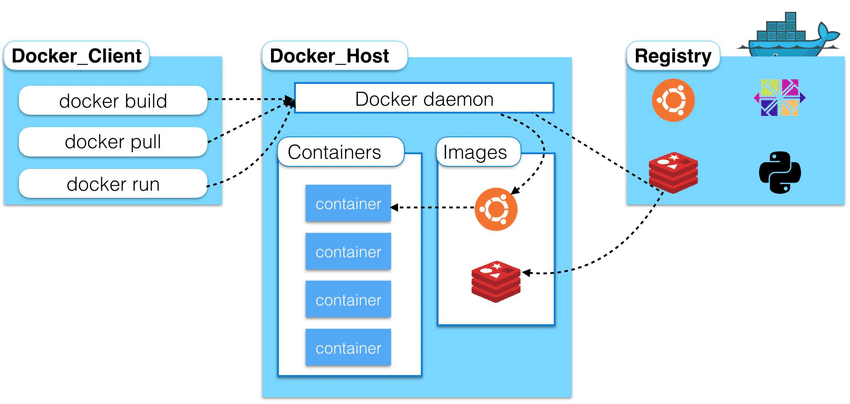
\includegraphics[scale=0.3]{./pics/High-level-overview-of-Docker-architecture.jpg}
    \caption{Docker}
    \end{figure}
\end{frame}

%------------------------------------------------

\subsection{Docker Compose} 
\begin{frame}
\frametitle{Docker Compose}
\begin{block}{FROM}
This will import a base image.
\end{block}

\begin{block}{COPY}
This will copy files into the image.
\end{block}

\end{frame}

%------------------------------------------------

\begin{frame}
\frametitle{References}
\footnotesize{
\begin{thebibliography}{99} % Beamer does not support BibTeX so references must be inserted manually as below
\bibitem[Docker, 2018]{whatisdocker} Docker (2018)
\newblock What is Docker
\newblock \href{https://www.docker.com/what-docker}{https://www.docker.com/what-docker} 
\end{thebibliography}
}
\end{frame}

%------------------------------------------------

\begin{frame}
\Huge{\centerline{The End}}
\end{frame}

%----------------------------------------------------------------------------------------

\end{document}